\chapter{Normal operations}
\thispagestyle{fancy}
\minitoc[n] % Creating an actual minitoc

\section{Airspeed Normal Operations}
\begin{table}[h]
\caption{Airspeed for Normal Operations}
\label{tab:airspeed_normal}
  \begin{tabularx}{\linewidth}{
    |>{\hsize=0.2\hsize}X| 
     >{\hsize=0.6\hsize}X|
     >{\hsize=0.2\hsize}X| 
} 
 \hline % These need to be measured for this aircraft
  Symbol & Description &  Airspeed \\ 
 \hline
 $V_{r}$ & Take off rotate speed & 70 kt\\ 
 \hline
 $V_{x`}$ & Best angle of climb & 74 kt  \\ 
 \hline
 $V_{y}$ & Best rate of climb & 104 kt \\ 
 \hline 
  $V_{fe}$ & Maximum full flap speed & 87 kt\\ 
 \hline 
  $V_{fe20}$ & Maximum 20$^{\circ}$ flap speed & 96 kt\\ 
 \hline
 $V_{a}$ & Manoeuvering speed (no full or abrupt control movement) & 123 kt\\
 \hline
 $V_{no}$ & Turbulent air operating speed & 168 kt\\ 
 \hline
 $V_{ne}$ & Never exceed speed & 200 kt\\ 
 \hline
 $V_{ref}$ & Landing final approach full flap & 70 kt\\ 
 \hline
 $V_{gl}$ & Best glide & 78 kt\\ 
 \hline
 $V_{s}$ & Stall flapless  & 55 kt \\ 
 \hline
 $V_{so}$ & Stall full flap & 51 kt\\ 
 \hline
\end{tabularx}
\end{table}

\begin{figure}[h]
\centering
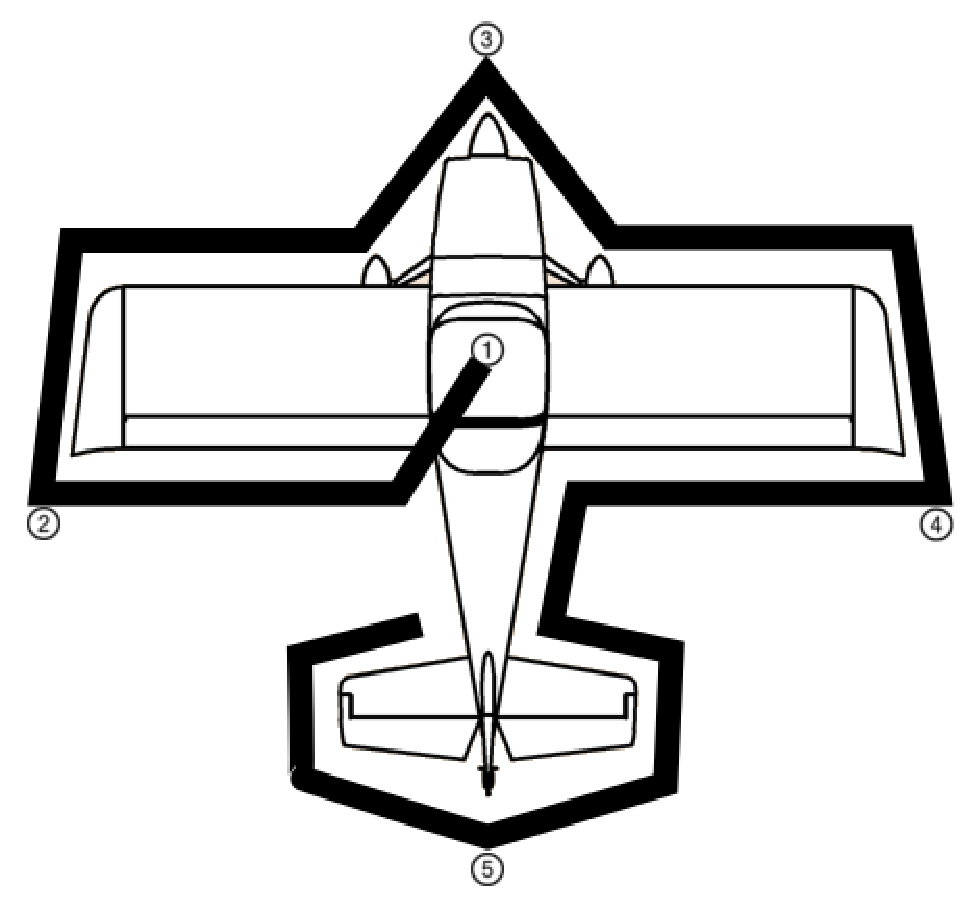
\includegraphics[height=0.5\textheight]{walkaround2.eps}
\caption{Walkaround}
\label{fig:walkaround}
\end{figure}

\section{Before Entering the Airplane}
%\begin{enumerate}[\circled{1}]
\circled{1}
\begin{enumerate}[(1)]
\item Master and EFIS (backup power) -- ON
\item EFIS runs off backup power -- CHECK
\item EFIS power from main -- ON
\item Fuel gauges -- CHECK
\item Flaps -- EXTEND FULLY
\item Master and EFIS -- OFF
\end{enumerate} 	
\circled{2}
\begin{enumerate}[(1)]
\item Left wing control surfaces -- CHECK
\item AoA port -- CLEAR
\item Pitot tube -- CLEAR
\item Left tank -- CHECK LEVEL and CAP SECURE
\item Left strainer -- DRAIN and CHECK
\item Left wheel -- CHECK
\end{enumerate}
\circled{3}
\begin{enumerate}[(1)]
\item Fuel vents -- CLEAR
\item Windshield -- CLEAN and SECURE
\item Air inlets -- CLEAR
\item Prop and Spinner -- CHECK
\item Oil -- Check level (~6 Qt)
\item Cowls -- SECURE
\end{enumerate}
\circled{4}
\begin{enumerate}[(1)]
\item Right tank -- CHECK LEVEL and CAP SECURE
\item Right strainer -- DRAIN and CHECK
\item Right wing control surfaces -- CHECK
\item Right wheel -- CHECK 
\end{enumerate}
\circled{5}
\begin{enumerate}[(1)]
\item Static port -- CLEAR
\item Rear Empennage Fairing -- CHECK
\item Elevator -- CHECK
\item Rudder -- CHECK
\item Tail wheel -- CHECK
\end{enumerate}

\section{Before Starting the Engine}
\begin{enumerate}[(1)]
  \item Seats and Seat Belts -- Adjust and Lock
  \item Alternate air -- OFF (Emergency use only)
  \item Brakes -- Test
  \item Avionics -- OFF
  \item Flaps -- RETRACT IN STAGES ($40^\circ, 30^\circ, 15^\circ, 0^\circ$)
\end{enumerate}

\section{Priming the Engine (Cold Engines Only)}
\begin{enumerate}[(1)]
  \item Propellor -- FINE
  \item Fuel valve -- SELECT
  \item Master -- ON
  \item EFIS -- ON
  \item Fuel pump -- ON
  \item Throttle -- OPEN FULL
  \item Mixture -- ADVANCE TO FULL RICH (Until slow but steady fuel flow achieved for 3-5s)
  \item Throttle -- CLOSED
  \item Mixture -- IDLE CUT OFF
  \item Fuel pump -- OFF
\end{enumerate}

\section{Starting Engine (Cold)}
\begin{enumerate}[(1)]
  \item Prime -- AS REQUIRED
  \item Throttle -- OPEN 1/4 TRAVEL
  \item Ignition Switch -- START (release when engine starts)
  \item Mixture -- FULL RICH (slowly and smoothly)
  \item Throttle -- SET 1000 RPM
  \item Oil Pressure -- CHECK (stop if not green in 30s)
  \item Ammeter -- ON AND CHARGING
  \item Mixture -- LEAN (for taxi)
  \item Avionics -- ON 
\end{enumerate}

\section{Starting Engine (Hot)}
\begin{center}
NOTE

Do not move mixture from its FULL CLOSED position prior to a hot start.
\end{center}
\begin{enumerate}
  \item Mixture -- FULL LEAN
  \item Throttle -- FULL OPEN
  \item Inition -- ON
  \item Ignition Switch -- START (release when engine starts)
  \item Mixture -- FULL RICH (slowly and smoothly)
  \item Throttle -- CLOSE AND SET 1000 RPM
  \item Ammeter -- ON AND CHARGING
  \item Mixture -- LEAN (for taxi)
  \item Avionics -- ON 
\end{enumerate}

\section{Ground Running and Warm-up}
\begin{enumerate}[(1)]
  \item Aircraft -- Into Wind
  \item Mixture -- RICH
  \item Propellor -- FINE
  \item Throttle -- SET 1000-1200 RPM (less than 2200 RPM on ground)
\end{enumerate} 

%\begin{center}
%NOTE

%Engine is warm enough when throttle can be opened without %faltering.
%\end{center}

\section{Power Check}
\begin{enumerate}[(1)]
  \item Brakes -- ON
  \item Fuel selector -- SWITCH
  \item Oil Temperature -- GREEN
  \item Oil Pressure -- GREEN
  \item Mixture -- RICH
  \item Throttle -- 1000 - 1500  RPM
  \item Propellor -- CYCLE x 3 (Avoid more than 500 RPM drop)
  \item Throttle -- SET 1800 RPM (50-65\% power)
  \item Magneto -- CHECK (175 drop 50 RPM difference)
  \item Alternate air -- Check for RPM drop on activation
  \item Engine instruments and Ammeter -- CHECK 
  \item Flights Instruments and Radios -- SET
  \item Beacon, Navigation lights -- ON (as required)
  \item Wing Flaps - CHECK 
\end{enumerate} 

\begin{center}
NOTE
 
Any ground check that requires full throttle operation must be limited to three minutes, or less if the cylinder head temperature should exceed the maximum as stated in this manual.
\end{center}

\section{Take Off}
\subsection{Normal Take Off}
\begin{enumerate}[(1)]
  \item Flaps -- UP
  \item Throttle -- OPEN 
  \item Mixture -- RICH (lean for field elevation)
  \item Rotate -- 70 KIAS
  \item Climb Speed -- $V_y$ 104 KIAS 
\end{enumerate}
\subsection{Maximum Performance Take Off}
\begin{enumerate}[(1)]
  \item Flaps -- 15$^{\circ}$
  \item Brakes -- APPLY
  \item Throttle -- FULL THROTTLE  
  \item Mixture -- RICH (lean for field elevation)
  \item Brakes -- RELEASE
  \item Rotate -- 55 KIAS
  \item Climb Speed -- $V_x$ 74 KIAS 
  \item Wing Flaps -- RETRACT after reaching 74 KIAS
\end{enumerate}
\begin{center}
NOTE

Do not reduce power until wing flaps have been retracted.
\end{center}

\section{Enroute Climb}
\begin{enumerate}[(1)]
  \item Airspeed -- $V_y$ 104 KIAS or higher
  \item Power -- 25 INCHES or FULL THROTTLE and 2500rpm 
  \item Mixture -- LEAN as required
\end{enumerate}

\section{Cruise}
\begin{enumerate}[(1)]
\item Power -- 15-25 INCHES, 2100 - 2500 RPM (no more than 75\%)
\subitem Performance (75\% Power): RPM 2450, Fuel Flow 12.3 Gal (47l/h) %~10gal 48 liters/h
\subitem Economy (65\% Power): RPM 2350, Fuel Flow 9.5 Gal (36l/h) %8.66 ~33l/h
\item Mixture -- LEAN as required
\end{enumerate}

\section{Before Landing}
\begin{enumerate}[(1)]
\item Mixture -- RICH
\item Propeller -- HIGH RPM
\item Airspeed -- 70-80 KIAS (flaps UP)
\item Wing Flaps -- As Required (20$^{\circ}$below 96 KIAS 20$^{\circ}$-40$^{\circ}$ below 87 KIAS)
\item Airspeed -- 60-70 KIAS (flaps DOWN)
\end{enumerate}

\section{Balked Landing (Go-around)}
\begin{enumerate}[(1)]
\item Power -- FULL THROTTLE and 2700rpm
\item Wing Flaps -- RETRACT to 20$^{\circ}$
\item Airspeed --  70 KIAS
\item Wing Flaps -- RETRACT slowly
\end{enumerate}

\section{Engine Shutdown}
\begin{enumerate}[(1)]
\item Propellor -- FINE 
\item Throttle  -- IDLE until CHT drop
\item Mixture  --  IDLE CUT OFF
\item Master -- OFF when engine stops
\end{enumerate}

\section{Amplified Procedures}
%\subsection{Power checks}

\subsection{Before starting engine}
When testing the brakes both brake pedals should have a similar feel and a firm resistance after 1/2" of pedal travel.

\subsection{Throttle operation}
Throttle movements from full power to idle or from idle to full power are full range movements. Full range throttle movements must be performed over a minimum time duration of 2 to 3 seconds. Performing a full range throttle movement at a rate of less than 2 seconds is considered a rapid or
instant movement. Performing rapid movements may result in detuned counterweights which may lead to failure of the counterweight lobes and subsequent engine damage.


\subsection{Take off}
The auxiliary fuel pump is normally off during take offs.  If there is evidence of fuel vapour or rough engine operation the pump should be turned on.

Full throttle runups over loose gravel are harmful to propeller tips.  Rolling take offs where the throttle is advance gently is suggested.  

Use full-rich mixture during takeoff or climb. Careful observation of engine temperature instruments should be practiced to ensure the limits specified are never exceeded.
Prior to take off from fields above 3000 ft elevation the mixture should be leaned.


\subsection{Wing flap settings}
Check that the flaps are retracted evenly. When flap is needed to shorten take off runs, no more than 15$^{\circ}$ is suggested.

\subsection{Enroute climb}
Normal climbs are performed with the flaps retracted and the airspeed 5 to 15 kt faster than best rate of climb speed.  Power selected should not be less than 25" MAP and 2500 rpm. Full throttle climb at 2400 RPM and higher is allowed. 

\subsection{Cruise}
Normal cruising is performed between 55\% and 75\% power.  
For reduced noise levels the lowest RPM in the green arc for the desired power setting is suggested.

For maximum service life, maintain the following limits are recommended for continuous cruise operation:\\
\begin{itemize}
\item Engine power setting - 65\% of rated or less.
\item Cylinder head temperatures - 400$^{\circ}$F or below.
\item Oil temperature 165$^{\circ}$F to 220$^{\circ}$F.
\end{itemize}
\begin{center}
NOTE\\

After engine rework cruising should be done at 65\% to 75\% power for 50 hours or until oil consumption stabilise.
\end{center}

\subsection{Mixture leaning in flight}
The relationship between Mixture setting and engine power is indicated in Figure~\ref{fig:Leaning_graph}.

\begin{figure}[H]
\centering
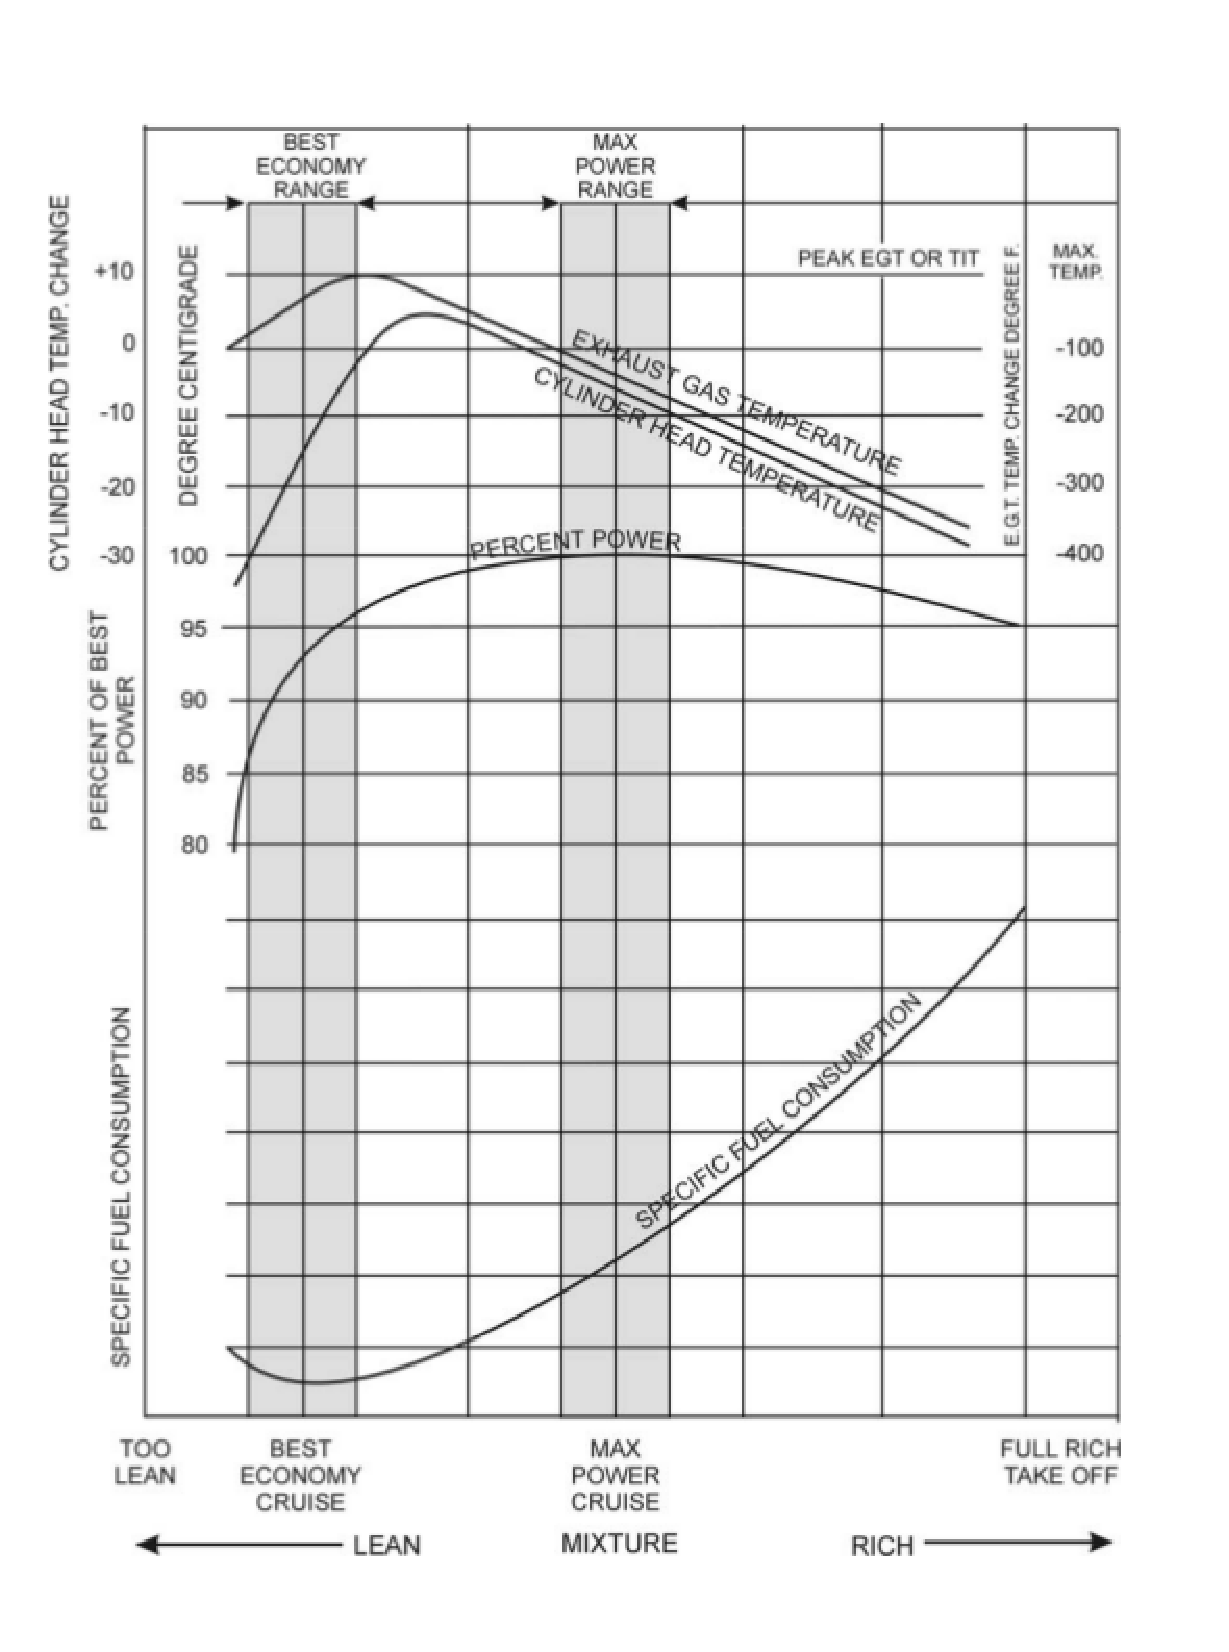
\includegraphics[height=0.8\textheight]{Leaning_graph.eps}
\caption{Lycoming power leaning curve}
\label{fig:Leaning_graph}
\end{figure}

\subsection{Leaning with Exhaust Gas Temperature (EGT) Gauge}
\subsubsection{Maximum Power Cruise}
\begin{enumerate}[(1)]
\item Approximately 75\% Power.
\item Never lean beyond 150$^{\circ}$ on RICH side of peak EGT.
\item Monitor cylinder head temperatures.
\end{enumerate}

\subsubsection{Best Economy Cruise}
\begin{enumerate}[(1)]
\item Approximately 75\% Power and BELOW.
\item Operate at PEAK EGT.
\end{enumerate}

\subsection{Leaning with Manual Mixture Control}
Economy cruise, 75\% power or less, without flowmeter or EGT gauge
\begin{enumerate}[(1)]
\item Slowly move mixture control from FULL RICH position toward lean position.
\item Continue leaning until slight loss of power is noted\\ (loss of power may or may not be accompanied by roughness.)
\item Enrich until engine runs smoothly and power is regained.
\end{enumerate}

\subsection{Let down}
Sudden cooling is detrimental to the good health of the aircraft engine. Lycoming Service Instruction 1094D recommends a maximum temperature change of 50${^\circ}$F per minute to avoid shock cooling of the cylinders.

Pilots must avoid fast letdowns with very low power (high-cruise RPM and low manifold pressure), along with rich mixtures that contribute to sudden cooling. It is recommended that pilots maintain at least 15" MAP or higher, and set the RPM at the lowest cruise position. 

Letdown speed should not exceed high cruise speed or approximately 1,000 feet per minute of descent. Keeping descent and airspeed within these limits will help to prevent the sudden cooling that may result in cracked cylinder heads, warped exhaust valves, and bent push rods.

The mixture setting also has an effect on engine cooling. To reduce spark plug fouling and keep the cylinder cooling within the recommended 50${^\circ}$F per-minute limit, the mixture should be left at the lean setting used for cruise and then richened gradually during the descent from altitude. The lean mixture, maintaining some power and using a sensible airspeed should achieve the most efficient engine temperatures possible.

\subsection{Crosswind Landing }
When landing in a crosswind, use the minimum flap setting required for the field length available.

\subsection{Go-around }
In a go-around, apply full throttle and 2700 RPM smoothly using fine pitch.  Reduce wing flaps promptly to climb setting.   Upon reaching a safe airspeed with positive rate of climb flaps should be retracted fully.

\subsection{Cold Weather Operation}
Prior to starting in cold temperatures it is advisable to pull the propeller through several times.  

\begin{center}
NOTE\\

When pulling through the propeller treat it as if the ignition is on.  A loose or broken ground wire to either magneto could cause the engine to fire.
\end{center}

\section{Aerobatic Flight}
\subsection{Aerobatic Flight}
The aircraft is capable of easily performing basic aerobatic manoeuvres. This capability is due to its relatively high power loading and aerodynamic cleanliness which produces the speed or energy needed.  Excessive speed build-up can occur very quickly and should be of primary concern when attempting and practicing aerobatics.  Elevator stick forces are relatively light, over stressing could easily occur.  Pilots should received formal aerobatic training before attempting aerobatic flight.

\subsection{Airspeed Aerobatic Manoeuvres}
The aircraft is capable of performing the aerobatic manoeuvres listed in Table~\ref{tab:aero_speeds}.

\begin{table}[h]
\caption{Aerobatic Entry Speeds}
\label{tab:aero_speeds}
  \begin{tabularx}{\linewidth}{|
    >{\hsize=0.6\hsize}X|
    >{\hsize=0.2\hsize}X|
    >{\hsize=0.2\hsize}X|
  }
\hline
Manoeuvre: & Speed \newline Minimum & Speed \newline Maximum\\
\hline
Loops, Horizontal eights:&122 kt &  165 kt\\
\hline
Immelman Turns: & 130 kt& 165 kt\\
\hline
Aileron Rolls, Barrel Rolls: &104 kt& 165 kt\\
\hline
Snap rolls &70 kt& 96 kt\\ 
\hline
Vertical Rolls: & 156 kt & 165 kt\\
\hline
Split-S:       & 87 kt&  96 kt\\
\hline
\end{tabularx}
\end{table}

 
